\documentclass[11pt]{article}

\usepackage{natbib}
\usepackage{aas_macros}
\usepackage{hyperref}
% \usepackage{aasmacros}
% \usepackage{geometry}                % See geometry.pdf to learn the layout options. There are lots.
%\geometry{a4paper}                   % ... or a4paper or a5paper or ... 
%\geometry{landscape}                % Activate for for rotated page geometry
%\usepackage[parfill]{parskip}    % Activate to begin paragraphs with an empty line rather than an indent
\usepackage{graphicx}
\usepackage{amssymb}
%\usepackage{epstopdf}
%\DeclareGraphicsRule{.tif}{png}{.png}{`convert #1 `dirname #1`/`basename #1 .tif`.png}

\title{Optical interferometry}
\author{Staff contact: Grant Kennedy}
\date{}                                           % Activate to display a given date or no date

\begin{document}
\maketitle

\tableofcontents

\section{Introduction}

You are probably familiar with Young's double slit experiment, where light from a single monochromatic point source (commonly a laser) passes through two slits and forms ``fringes'' on a screen or detector. The spacing of these fringes is $\lambda/b$, where $\lambda$ is the wavelength of the light, and $b$ the distance between the slits. The bright fringes are where the path lengths from the two slits are an integer number of wavelengths, so the light constructively adds, and the dark fringes are where the paths differ by half of the wavelength of the light, and so cancel.

There is a somewhat obvious question to ask of this experiment; what happens if the source is not a point? One reason this is obvious is that sources are never really points, and have some finite size. For example, we can for most purposes consider stars to be point sources because their angular size is very small compared to the resolution of typical telescopes, but given sufficient angular resolution this assumption is not true.

A finite source size fundamentally changes the double slit experiment as we normally encounter it. Consider a second point source of equal brightness that is incoherent with the first, and that is located at an angle $\lambda/(2b)$ away. The two fringe patterns are $180^\circ$ out of phase so will cancel, leaving a uniformly illuminated detector with half of the peak brightness.

While either source would individually produce a set of fringes, together their fringes add to produce none, and this difference is the result of the spatial separation of the two sources. That is, the double slit experiment therefore provides a means to infer spatial information about sources by measuring fringe patterns. Here we will be concerned with the fringe amplitudes, which are also known as ``fringe visibilities'' or simply ``visibilities''. Though we will not be concerned with them here, the phases are also important, primarily giving information regarding spatial location (e.g. consider how the fringes in the single source case move as the source is moved to one side; the amplitude remains the same but the phase changes).

The first use of such an ``interferometer'' in astronomy was to measure the size of the moons of Jupiter \citep{1891PASP....3..274M,1891Natur..45..160M}, and 30 years later the technique was used to measure the diameter of another star \citep{1921ApJ....53..249M}. Interferometry is now a widely used technique in astrophysics, and is normally concerned with measuring the sizes of small objects, or with obtaining images of objects and structures that have relatively small angular scales.

What does ``small'' mean here? As we saw above, when the separation between two point sources is $\lambda/(2b)$, the fringes disappear (the visibility is zero). The angular resolution of an interferometer is therefore defined as $\lambda/(2b)$, where $b$ is the distance between two telescopes, that serve the same purpose as the slits in the double slit experiment. Compare this to Rayleigh's criterion, $1.22 \lambda/D$, where $D$ is the diameter of the aperture or telescope. Now if $D$ and $b$ are similar the resolution of an interferometer and a normal ``single-dish'' telescope is similar. But there is one key difference; the space between the two telescopes of an interferometer can be empty, meaning that it is practically much easier and cheaper to make $b$ large (e.g. tens/hundreds of meters for optical wavelengths, and kilometers for millimeter wavelengths) than it is to make $D$ large. The largest single-dish telescopes we have are of order tens (optical) to hundreds (radio) of meters.

Thus, the key thing an interferometer does is allow us to make measurements on small angular scales, without constructing a single-dish telescope that would do so based on Rayleigh's criterion. In this experiment you will use exactly the same methods used in optical interferometry, just on a smaller scale.

\clearpage
\section{Theory}

This experiment is little more than an extension of Young's double slit experiment. The only real difference is that we will be using an extended source that is incoherent. Typically the double slit experiment uses a coherent point source (e.g. a laser). Here the slits will also be replaced with pairs of holes, so instead of the usual one-dimensional picture, fringes are spread over a two-dimensional plane with an orientation that depends on the orientation of the holes. 

\begin{figure}[h]
    \centering
    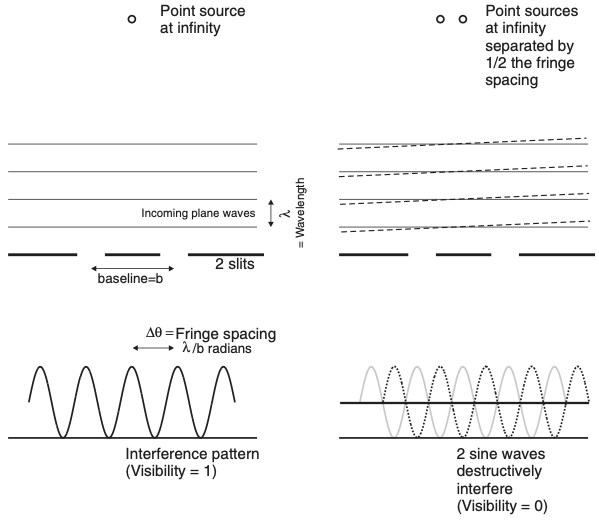
\includegraphics[width=0.8\textwidth]{doc/youngs.png}
    \caption{Illustration of Young's double slit experiment (\emph{left}), and the resulting intensity image when two point sources are observed (\emph{right}). Credit: \citet{2003RPPh...66..789M}.}
    \label{fig:youngs}
\end{figure}

To recap the double slit experiment, Figure \ref{fig:youngs} shows the expected fringe pattern for a point source at infinity and with slits that have a spacing $b$. In interferometry, this separation is commonly called a ``baseline''. We assume that we are observing light that has a limited range of wavelengths that is centered on $\lambda$. The fringe pattern then has a spacing of $\lambda/b$; this is the angle in radians between fringe peaks from the plane of the slits to the detector. The fringe pattern intensity $I$ is commonly written as
\begin{equation}\label{eq:fringepattern}
    I = 4 I_0 \cos^2 \frac{\delta}{2}
\end{equation}
where $I_0$ is the intensity that would have resulted from light passing through a single hole or slit, and where $\delta$ is the phase difference that results from the different path lengths from the slits to a given point on the detector.

Now consider a second source of equal brightness, with an angular separation from the first of $\lambda/(2b)$. The fringes produced by this source will be 180$^\circ$ out of phase compared to the fringes from the first source, so will cancel. Because we are considering an analogy with an astronomical observation, the two sources are expected to be incoherent because their spatial separation will typically be large (e.g. thousands of km apart on the surface of a star) and there is no reason to believe there is any laser-like behaviour that synchronises photon phases, so the phases of two photons coming from the two sources will have random phases with respect to each other. Thus, at any point on the detector we can simply add the intensity from the two independent fringe patterns (there is no sustained interference between the two patterns). For the case with the second source separated by $\lambda/(2b)$, the result is therefore no fringes at all, as shown in the right panel of Figure \ref{fig:youngs}. This disappearance of the fringes is how we define the resolution of an interferometer, while for single-dish (normal) telescopes with diameter $D$ it is the Rayleigh criterion of 1.22\,$\lambda/D$, for interferometers it is $\lambda/(2b)$.

\begin{figure}[h!]
    \centering
    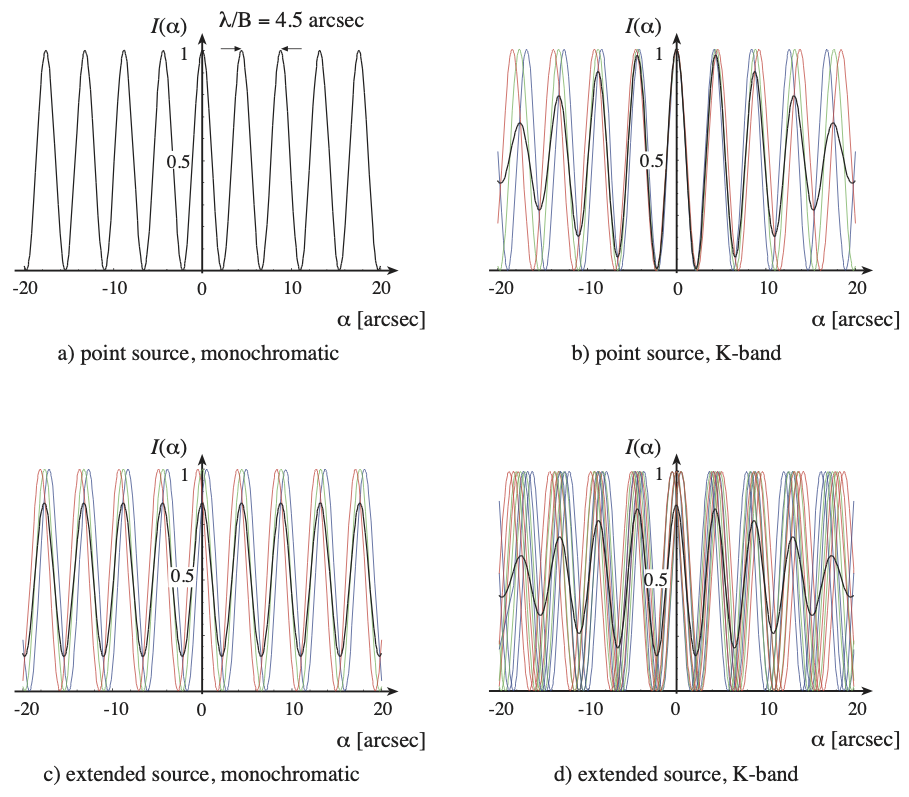
\includegraphics[width=1\textwidth]{doc/coherence.png}
    \caption{Illustration of how the fringe pattern is altered by a finite range of wavelengths and an extended source size (assuming a baseline of 10\,cm). Each panel shows several of the fringe patterns that are being superimposed, which result in the overall pattern shown as the thicker black line. The top left panel shows the fringe pattern for a monochromatic point source, and the other panels show how the fringe amplitude is reduced. The top right shows the effect for a range of wavelengths in the `K' band (near 2.5\,$\mu$m). The lower left panel shows the effect for an extended source, and the lower right panel the combination of an extended source and range of wavelengths. Credit: \href{https://www.eso.org/sci/facilities/paranal/telescopes/vlti/tuto/tutorial_spatial_interferometry.pdf}{Andreas Glindemann/ESO}}
    \label{fig:coherence}
\end{figure}

In intermediate cases where a second source is less separated, e.g. at $\lambda/(4b)$, the fringe patterns do not add up to a constant, but the amplitude of the pattern is still reduced. The same behaviour is typically observed when the source is extended, e.g. a uniform disk such as a stellar surface, since this case can be considered as the summation of a series of point sources. This reduction in fringe amplitude is illustrated in Figure \ref{fig:coherence}, most importantly in the lower left panel which considers a finite continuous source. A finite range of wavelengths will also reduce the fringe amplitude, though in this experiment we will reduce this effect by using filters to restrict the range of wavelengths.

In interferometry we are primarily interested in the amplitude of the fringes formed on our detector. We characterise this amplitude with the ``visibility'', which is defined as
\begin{equation}
    V = \frac{I_{\rm max} - I_{\rm min}}{I_{\rm max} + I_{\rm min}} \, .
\end{equation}
Looking at Figure \ref{fig:coherence}, we can see that the fringes in the top left panel have $V=1$ (and in the left panel of Figure \ref{fig:youngs}). For resolved sources the visibility is lower, for example in the lower left panel the value is about 0.6. For the right panel in Figure \ref{fig:youngs} the visibility is zero. Depending on how we measure it, a finite wavelength range will also lower the visiblity, as can be understood from the top right panel in Figure \ref{fig:coherence}.

In general, the fringes are an indication of how well ``resolved'' a source is. An unresolved source will have strong fringes and a high visibility, but as the source becomes more extended the fringes weaken and the visibility drops. For continuous sources as we will be considering here, which are analogous to the surface of a star for example, when the source is larger than about $\lambda/(2b)$ the visibility drops to near zero. This can be understood as the image on the detector being the superposition of many fringes that have such a wide range of phases that the average is a constant.

A more intuitive way to understand the origin of the visibility is that it is equal to the integral of the fringes as projected on the sky multiplied by the source. For the binary example with separation $\lambda/2b$, one source is on the peak of the fringe, while the other is on the minimum, so the integral is zero. An extended source, e.g. a star, that spans many fringes will have a low visibility, but one that is smaller than the fringe spacing will have a high visibility.

When making a measurement, we normally change the resolution of our instrument (i.e. the fringe spacing), either by changing the wavelength $\lambda$ or the baseline length $b$. A typical measurement therefore consists of making visibility measurements for a range of wavelengths and baseline lengths, and using these to infer spatial information about our source.

Note that as we are only using a pair of baselines, we are really only measuring the source size along an axis parallel with the baseline vector. For sources that are not rotationally symmetric, we can address this by rotating our baselines to a different angle with respect to the source and taking more measurements.

\subsection{Visibility functions}

Mathematically, we can write down the expected behaviour of the visibility as a function of baseline and wavelength for a few different source geometries. Some more detail on where these come from is given in \citet[][e.g. Fig 2.13]{2011psi..book.....G}.

The visibility for a binary source is perhaps not too surprising, we saw above that $V=1$ when their separation is zero, and $V=0$ when their separation is $\lambda/(2b)$, and $V$ varies sinusoidally in between. For a equal brightness binary with separation $s$, the visibility is
\begin{equation}
    V_{\rm binary} = \frac{1 + \cos ( 2 \pi s b / \lambda )}{2} \, .
\end{equation}

For an extended uniform circular source of diameter $\theta$ as a function of baseline length the visibility is
\begin{equation}
    V_{\rm uniform} = \frac{2 J_1(\pi \theta b / \lambda)}{\pi \theta b / \lambda} \, ,
\end{equation}
where $J_1$ is a first order Bessel function.

\begin{figure}
    \centering
    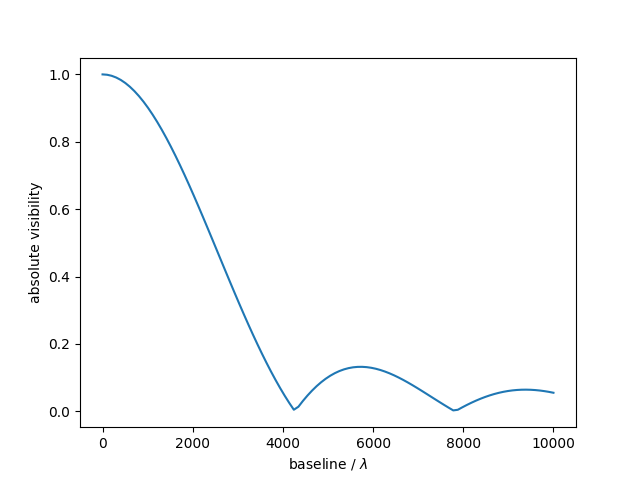
\includegraphics[width=0.8\textwidth]{doc/uniform_vis.png}
    \caption{Absolute visibility for a uniform source of 2\,mm diameter at a distance of 7\,m. For optical wavelengths the baselines are of order millimeters.}
    \label{fig:uniformvis}
\end{figure}

The latter is the visibility function that you will need for this experiment. To visualise either, the independent variable you are controlling is $b/\lambda$, so this should be the x-axis, and visibility is the quantity you are measuring, so this is the y-axis. As described above the uniform source therefore has decreasing visibility with increasing $b/\lambda$.

An example visibility curve for a uniform source is shown in Figure \ref{fig:uniformvis}. The y-axis plots the absolute value, as we only measure visibility in this experiment as a positive value (squared visibility is also commonly used). This plot is for a 2\,mm diameter source at 7\,m, which is similar to what you will use for this experiment. Likewise, the baselines are similar to this experiment, e.g. a 1\,mm baseline at 500\,nm is $b/\lambda=2000$.

\clearpage
\section{Experimental setup}

This lab has an intentionally simple setup; the goal is to show how one can construct an interferometer from a standard telescope with minor and straightforward modifications. The key pieces of equipment are:
\begin{itemize}
    \item Telescope, this is mounted to the bench and can be flipped up or down.
    \item CMOS detector and USB cable. Some information is \href{https://www.qhyccd.com/qhy5l-ii-planetary-guiding-camera/}{here}.
    \item Lens cap, this holds the tokens with the pairs of holes (baselines).
    \item Baseline tokens, these have small (0.3\,mm) holes drilled in pairs with a range of separations. These should be labelled, and the spacings are 0.6, 1, 2, 3, and 4\,mm.
    \item Light source. This is currently a bike light which has several brightness settings.
    \item Aperture tokens, these go in front of the light source and are what we observe. There are several sizes and shapes.
    \item Filters, used to change the wavelength of the source. You may take the mean wavelengths of these to be 448, 530, and 638\,nm for B, G, and R respectively. More detailed information is \href{https://www.firstlightoptics.com/rgb-filters-filter-sets/zwo-2-lrgb-filter-set.html}{here}.
    \item Miscellaneous fittings to mount the light source, aperture tokens, and filters.
    \item An ITS computer near the telescope, plug the CMOS into this one.
\end{itemize}

\subsection{Image capture software}\label{sec:software}

The software for this experiment is \href{http://www.firecapture.de/}{\texttt{FireCapture}}; it is an open source code primarily designed for amateur astronomers, and provides a friendly and easy to use interface for viewing images from the detector in real time, and allows saving of images in various formats.

A copy of the software will likely exist in \texttt{C://} on the computer near where the telescope is set up. If not, download the file to \texttt{C://}, unzip it and find the \texttt{FireCapture} application (within a second FireCapture folder) and double click it. It may ask if you want to unzip more files, if so say ``extract all'' and go with the suggested location. You will then need to open it again to run the software (and say yes to any queries about running/security).

You will probably be prompted to do some setup when you run \texttt{FireCapture} for the first time. Click the ``first time'' option; for most settings just leave the default, but select a new folder in which to save data on the ``capture'' options page. It would make sense to make another folder, e.g. \texttt{H://Interferometry/Data} for this, and if you use \texttt{H://} drive, you will have access to this from other ITS machines.

Having run the setup, a preferences file is saved in \texttt{C://Users/uXXXXXXX/FireCapture}. If you have problems, e.g. with the software crashing, try deleting this preferences folder and restarting \texttt{FireCapture}.

After the setup the software will go to a ``dummy camera'' that shows an image of Jupiter. Quit, and restart \texttt{FireCapture} when you have connected the detector (see setup steps below), at which point you should be prompted to select a detector, select \texttt{QHY}.

\begin{figure}[h]
    \centering
    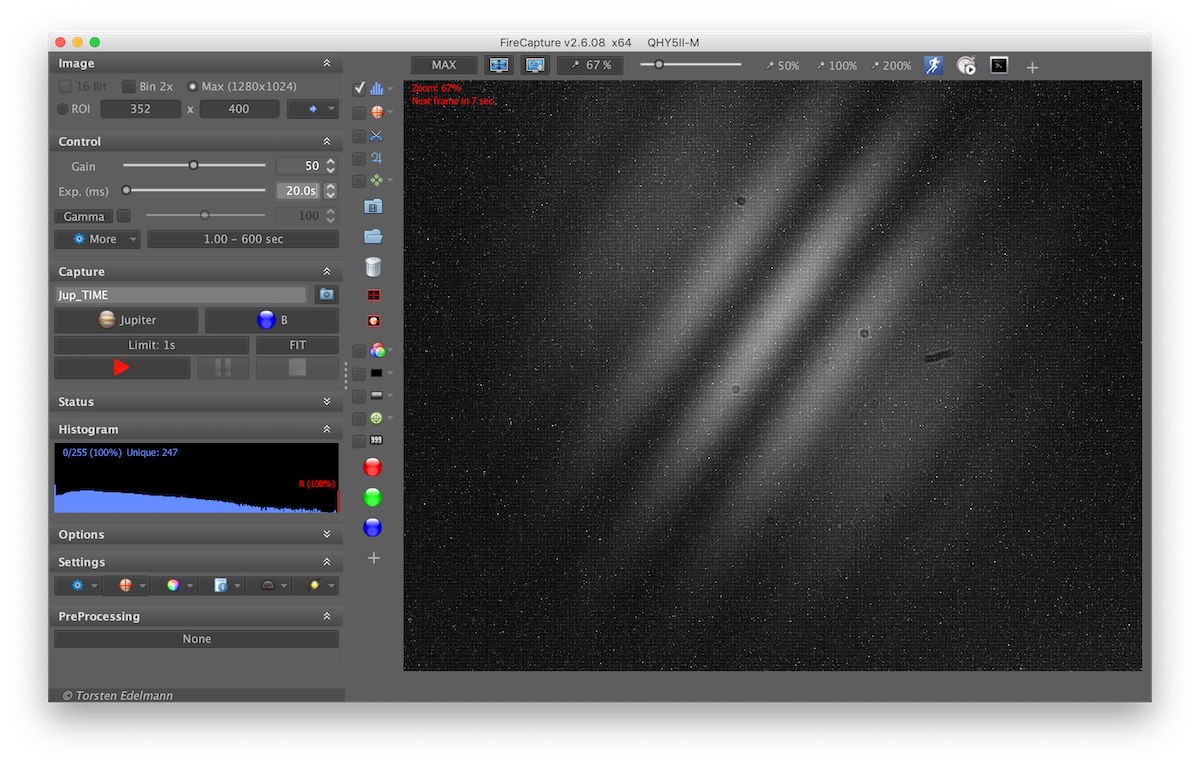
\includegraphics[width=1\textwidth]{doc/fc.png}
    \caption{Screenshot of the \texttt{firecapture} software running. The detector image is in the main panel, and various controls are in the left column.}
    \label{fig:fc}
\end{figure}

You will not need most of the options available in \texttt{FireCapture}. The main one in terms of obtaining images on screen is the exposure time (under ``control''); you will need to experiment, but values of about 1\,s are likely to be about right. The exposure time will however depend on what value you select for the gain. Higher gain images will require shorter exposures so be convenient when setting up, but will be noisier and introduce other artefacts, so it is better to take longer exposures at lower gain for measurements. You will know the exposure is appropriate when you have a clear image visible on screen, and this image is not saturated (the ``histogram'' panel may help here). There are some options above the image to set how the image is displayed, e.g. zoom, which you may wish to play with. In particular, the field of view may not initially be maximal; this can be changed by selecting ``Max'' rather than ``ROI'' (which is a definable sub-section of the detector). You can also optionally bin the images (average $2 \times 2$ sets of pixels), this will increase the signal to noise, but be careful not to degrade the image too much for longer baselines (shorter wavelength fringes).

The other important control is how images are saved (under ``capture''); for this you need to specify a directory in which to save images (if you didn't already at startup), a file format (select ``FIT''), and a number of images to save unde ``limit'' (just one, since you will hit save manually each time you change the baseline token, filter, etc.).

You can optionally save a ``dark frame'' (one of the small buttons between the main image and the left column of controls). For this cover the front of the telescope (putting your hand in front of the baseline token would suffice), and \texttt{FireCapture} will take an image that will be subtracted off subsequent images. The goal is that this dark image will contain any ``hot'' (permanently defective) detector pixels and other detector artefacts, and by subtracting them these pixels will not be visible in the final images. Ideally your dark frame will have the same settings as the images it is being subtracted from, as different settings (gain in particular) will result in different artefacts.

\subsection{Setup}

Setting up the experiment is reasonably simple, the aim being to have the telescope pointed at the light source and aperture. While having the telescope properly focused will aid the setup, it's not actually critical for observing the fringes. A suggested series of steps to get your first set up fringes is as follows:

\begin{enumerate}
    \item Plug the light source in to charge. The battery should last for hours, but it's best to turn it off when you're not using it.
    \item Ensure the telescope is in place with the lens cap on (no tokens needed yet).
    \item Insert the CMOS detector into the rear of the telescope and (gently) tighten the screws to keep it in place. You may end up rotating the detector later.
    \item Connect the CMOS detector to the computer with the USB cable.
    \item Open the image capture software (see \ref{sec:software}). The detector should be automatically recognised and an image appear on screen. Test whether the detector is working by removing/replacing the lens cap.
    \item Set up an aperture token at the other end of the lab using the mounting kit. Try to align the token such that the surface normal is pointing at the telescope.
    \item Remove the telescope lens cap and set up the focus and pointing. The telescope is fixed, so you will need to adjust the location of the aperture token until it appears near the center of the detector image. You will simultaneously need to adjust the focus so you know what you are pointing at. If you think the pointing is a long way off, you may find it helpful to hold a large object (e.g. a book) in front of the token to figure out where you need to point. You should end up with an in focus image of the aperture near the center of the detector.
    \item You may find it useful to orient the detector correctly, e.g. by placing a piece of paper near the source with an upwards pointing arrow on it, and rotating the detector so that the image on screen matches it. The orientation does not matter for rotationally symmetric sources.
    \item Set up the light source behind the aperture, fixing it to the bench with clamps. Point it towards the telescope. The pointing doesn't need to be too precise but the source and aperture should align reasonably well; you can test whether the source is pointing in the right direction by holding your hand in front of the aperture to see if the light is pointing towards the telescope. You can further check the alignment by decreasing the exposure time enough to see the source, and verify the the aperture is illuminated uniformly. Non-uniform illumination can result in unexpected results because the source size is not actually the size of the aperture.
    \item Insert one of the baseline tokens into the lens cap, preferably one of the shorter baselines. You should now see fringes on the detector with an image similar to Figure \ref{fig:det-img}, though may need to alter the exposure time (around 1\,s should be enough, though this will depend on gain and the source brightness setting).
\end{enumerate}

If all of this setup has gone well, you are now ready to start!

\clearpage
\section{Measuring visibilities}\label{sec:meas}

The key measurement in this experiment is of the fringe visibility. In the images this is essentially how strong the fringes are; if their amplitude covers the full range from peak to the background level the visibility is high (i.e. near 1), and if they are barely visible then the visibility is low (i.e. near zero).

\begin{figure}[h]
    \centering
    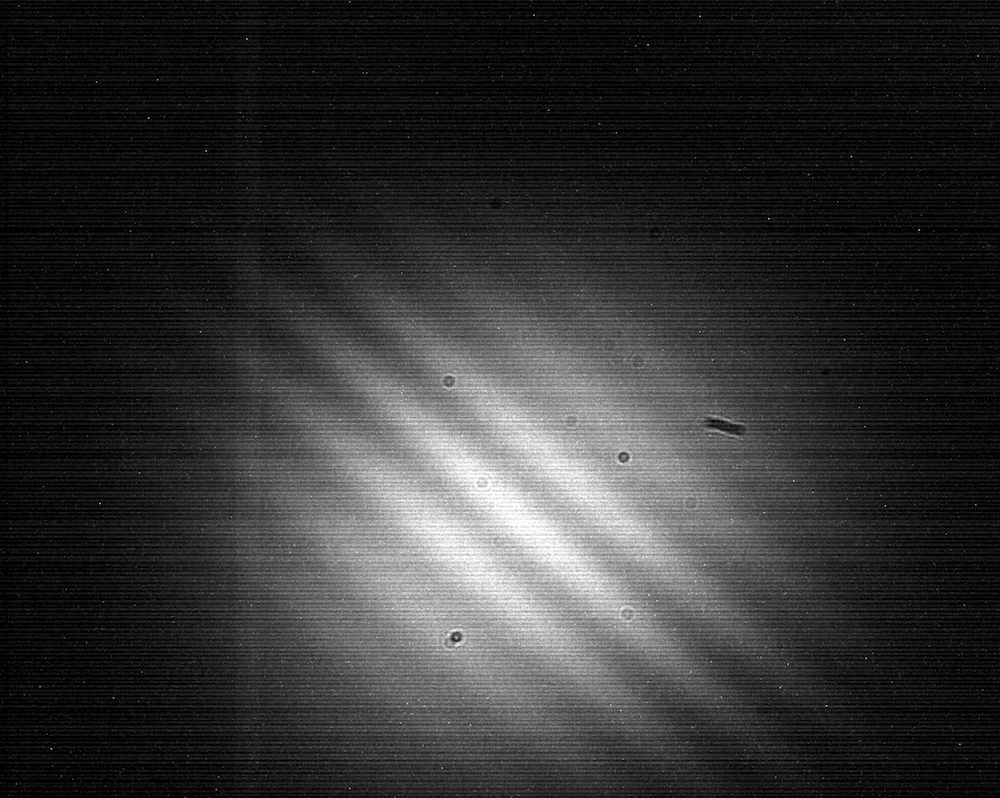
\includegraphics[width=0.8\textwidth]{doc/det-img.png}
    \caption{Example image. The broad circular envelope is the PSF, on which the fringes are superimposed. The small dots are artefacts from dust somewhere in the optical path, likely on the detector.}
    \label{fig:det-img}
\end{figure}

There are three components that contribute to an image, an example is shown in Figure \ref{fig:det-img}:
\begin{itemize}
    \item background; this is contributed by any stray light that reaches the detector, plus any intrinsic level attributed to the detector itself
    \item point spread function (PSF); this is the broad overall shape of the signal on the detector and is approximately Gaussian, and is set by the size of the individual holes in the baseline tokens. Smaller holes yield a larger diffraction pattern, and vice versa.
    \item fringes; this is the wavy pattern resulting from the pair of holes, the 2d version of the fringes from the experiment when done in 1d (e.g. with slits). The fringe orientation is set by the orientation of the holes (the fringes are perpendicular to a line between the holes), so can be used to quantify the orientation of the baseline token.
\end{itemize}
The goal in making a measurement is to subtract (or otherwise account for) the background, and make a measurement of the fringe visibility that (if possible/necessary) takes the shape of the PSF into account.

The simplest method for obtaining a visibility measurement would be to use the cursor in \texttt{FireCapture} to measure the background level somewhere away from the PSF, take peak and trough measurements for the fringes, subtract the background level from these, and then compute the visibility.

A more complex, but more reliable method, is to use the supplied python widget (\texttt{widget.py}); this code models the above components of the detector image to come up with a parameterised fit to the data, from which the visibility can be extracted. It can also make a visibility measurement using a Fourier transform.

There is no ``correct'' method here, and each method has its own problems. The image model does not account for the finite bandwidth, so fits poorly at longer baselines where the coherence is lower farther from the central fringes. This can be accounted for somewhat by ensuring the fit residuals look best near the peak. The Fourier method can be less reliable and is influenced by various factors, e.g. noisy images and image size (see Fourier example notebook). You should experiment, for example making measurements with all three methods and comparing the results. You should also consider how to incorporate uncertainties.

\subsection{Using \texttt{widget.py}}\label{sec:widget}

This code brings up an interactive window that allows a parameterised fit to a detector image, and which will output the model parameters, including the visibility and baseline angle (with respect to the detector, whose orientation depends on how you insert it into the telescope). The code itself exists on github, you can download it from
\href{https://github.com/drgmk/px-interferometry}{https://github.com/drgmk/px-interferometry} if it is not already on the machine you are using (have a look in \texttt{C://}). This software will be periodically updated, so check whether the version on the computer is up to date (e.g. by comparing file modification times and the last github commit date).

To run the python widget you can use either a system or python terminal. You can launch both of these from the \texttt{WinPython} install, which should be in \texttt{C://}. If you have issues, e.g. with python module errors, the solution is probably related to the \texttt{WinPython} version and a new version may need to be downloaded.

To run the widget from the shell directly, use
\begin{verbatim}
    python path/to/widget.py path/to/file.FIT 2
\end{verbatim}
The paths you enter will depend on where you run the command from.  The final argument (here 2) does $2 \times 2$ averaging to make the array for the image smaller so the fitting code runs faster. You could try 4 or higher, but if you average too much the detail in the image will be lost and the fit will be poor. A suggested approach is to use 4, but go to 2 if the fringes are very close together and the fit is not converging as well as you expect.

For the python terminal option, you first need to open a terminal, specifically the \texttt{WinPython PowerShell Prompt}. This will probably not open in the folder you want, so navigate to your data using the \texttt{cd} command. When you are at or near your data, run \texttt{ipython}, which will start a python terminal.

With the \texttt{python} terminal running, you will need to import and then run the code. To import, you need to add the widget location to your path, which if you can do with (adjusting the path as necessary).
\begin{verbatim}
    import os, sys
    sys.path.append(os.path.abspath(`C:/px-interferometry'))
\end{verbatim}
You can then import and run the widget with
\begin{verbatim}
    import widget
    widget.fit_fringes(`Data/FOLDERS/file.FIT',sc=2)
\end{verbatim}
where you will need to enter the correct path to the file you want to extract the visibility for. The option \texttt{sc=2} is the same as the final argument described above.

On running the widget a window will pop up with the image (FITS file), a model, an image of the residuals (image-model), and a cut through the center of the image perpendicular to the fringes in the model. An example is shown in Figure \ref{fig:widget}. The code will make an initial attempt to estimate the model parameters.

\begin{figure}[h!]
    \centering
    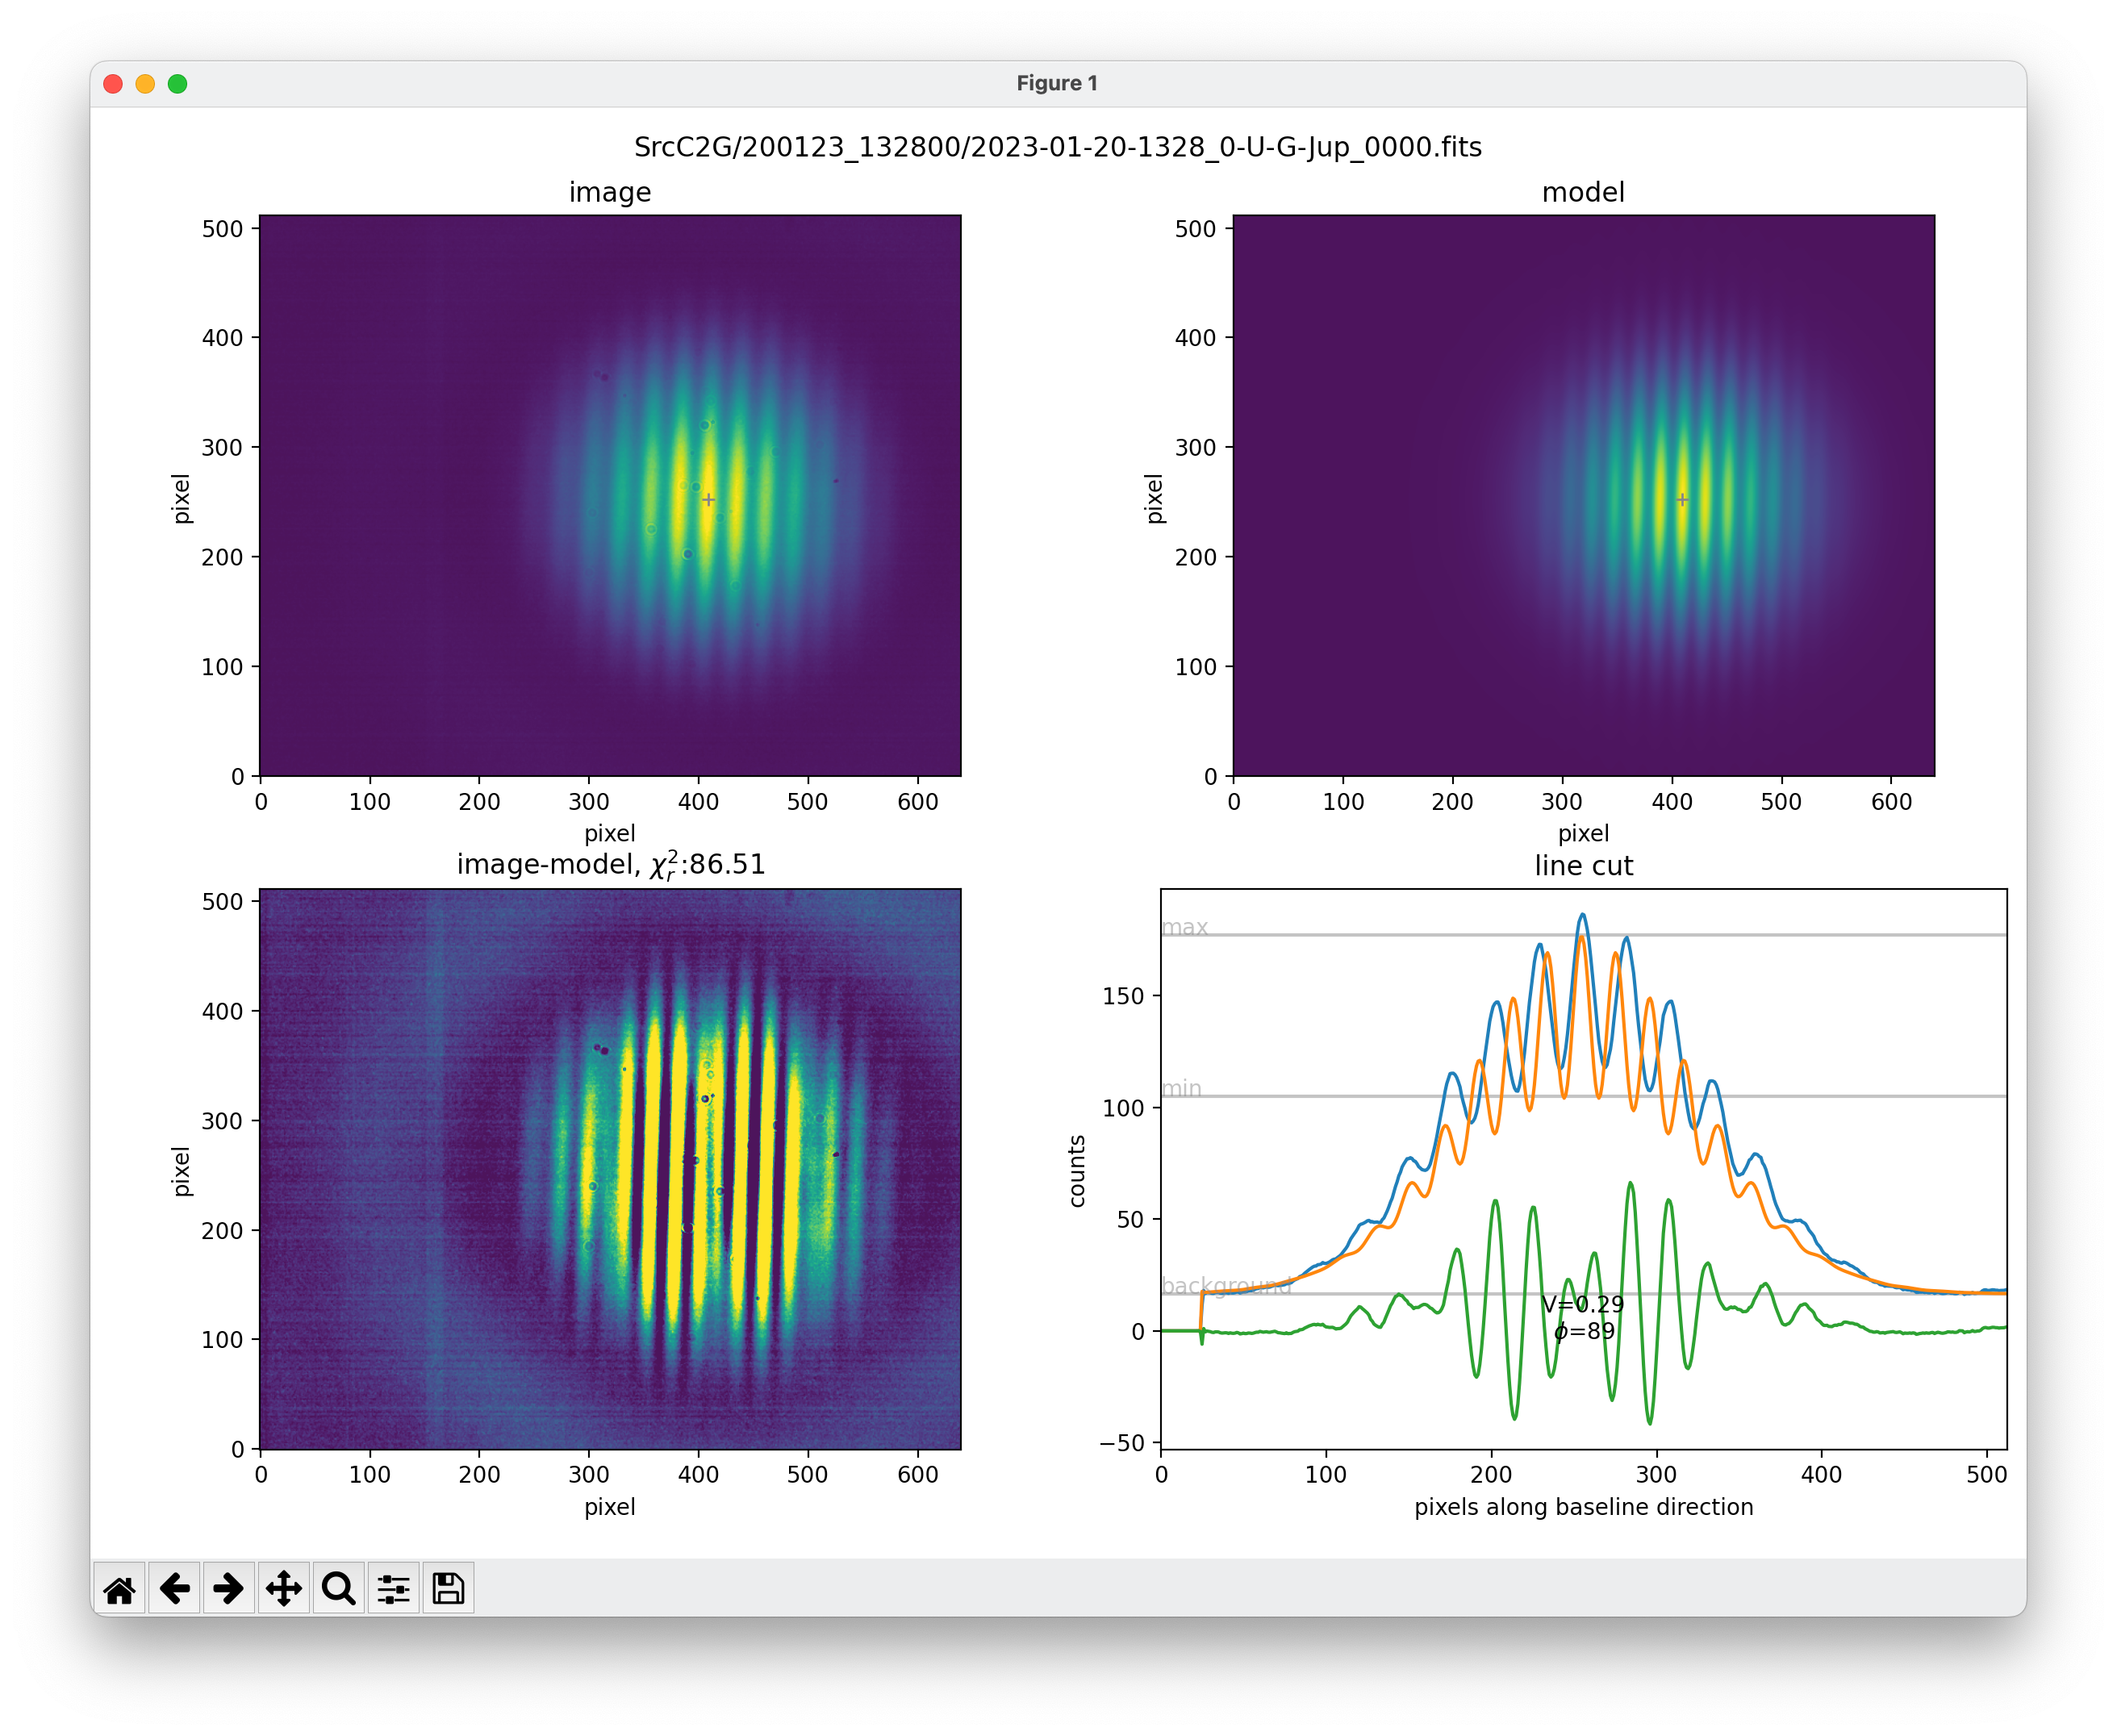
\includegraphics[width=1\textwidth]{widget.png}
    \caption{Example widget window. The top left panel shows the FITS image that is being fit. The top right shows the current model. The lower left shows the image-model residuals, and the lower right shows a cut through the image that is perpendicular to the model fringes (blue line), and the same cut through the model (orange line). This example shows the initial state, so the model does not fit the image at all well.}
    \label{fig:widget}
\end{figure}

The goal is then to improve the fit, which will almost certainly require some interaction. This works by moving the mouse cursor to a location on the image (top left panel), pressing a key on the keyboard to change some parameter, and repeating until the model is reasonably good. Details regarding keys can be found in the \texttt{widget.py} script. The fit can then be minimised (optimised) by pressing the \texttt{m} key. The residual plot may never look perfectly smooth, but the more uniform this image appears the better the fit. An example of a good fit is shown in Figure \ref{fig:widget2}. The results can be saved into a \texttt{numpy} save file with \texttt{S}, but the visibility is also shown as a number in the lower right panel. The advantage of saving your results in a file is that you can speed up the extraction, fitting, and plotting of the results with a systematic sequence of measurements. See the visibility notebook for an example.

\begin{figure}[h]
    \centering
    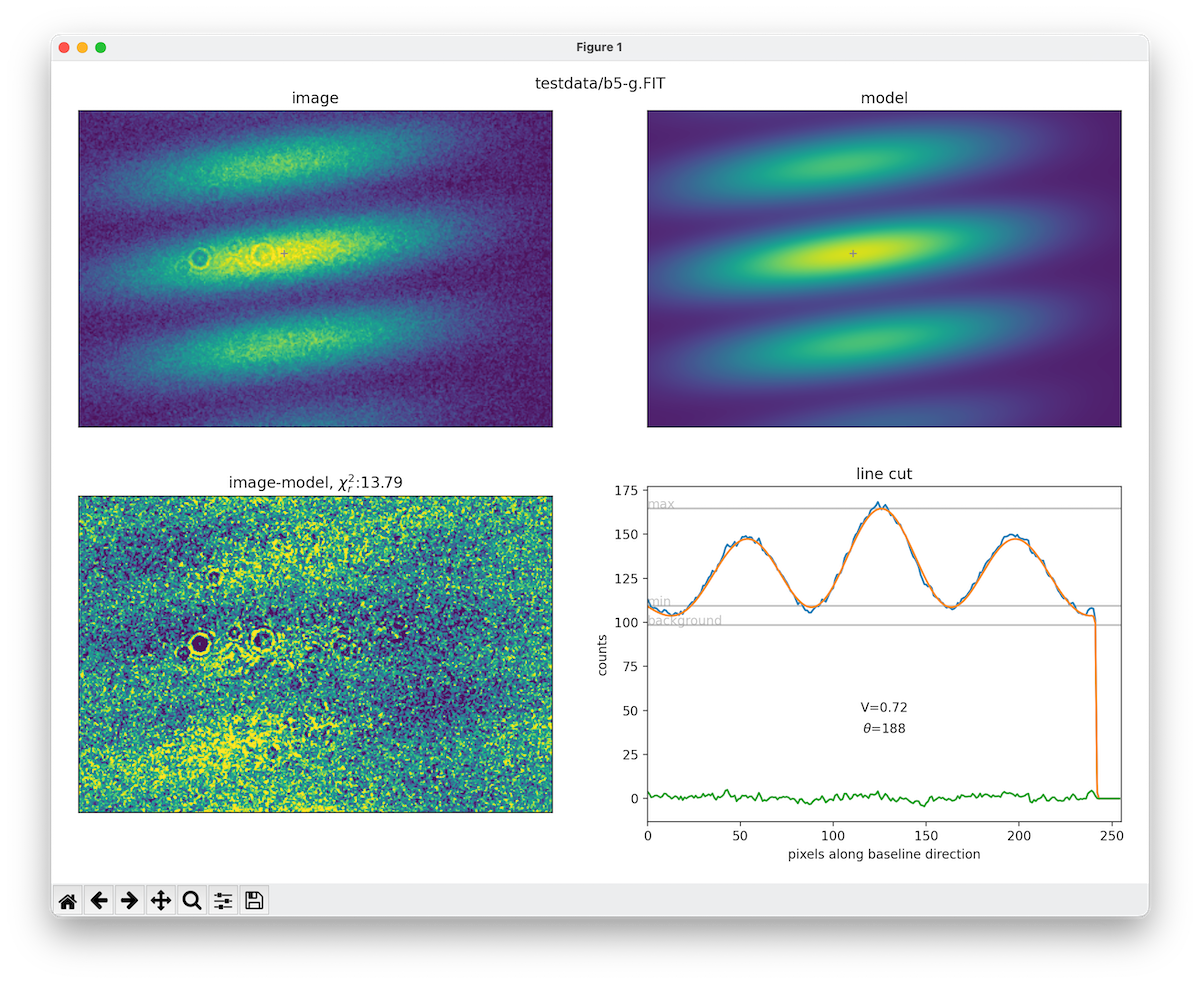
\includegraphics[width=1\textwidth]{widget2.png}
    \caption{Example widget window with a good model fit to the data.}
    \label{fig:widget2}
\end{figure}

\subsection{Fourier components}

The images obtained in this experiment are relatively simple, in that they have the three components of background, PSF, and fringes described above. This simplicity makes it possible to obtain information by Fourier transforming the images. We first subtract the background, so there are only two components. The Fourier transform then has only a broad PSF, and the narrower fringes, or thinking in terms of frequencies, some low frequencies that correspond to the PSF, and a single higher frequency that describes the fringes.

\begin{figure}[h]
    \centering
   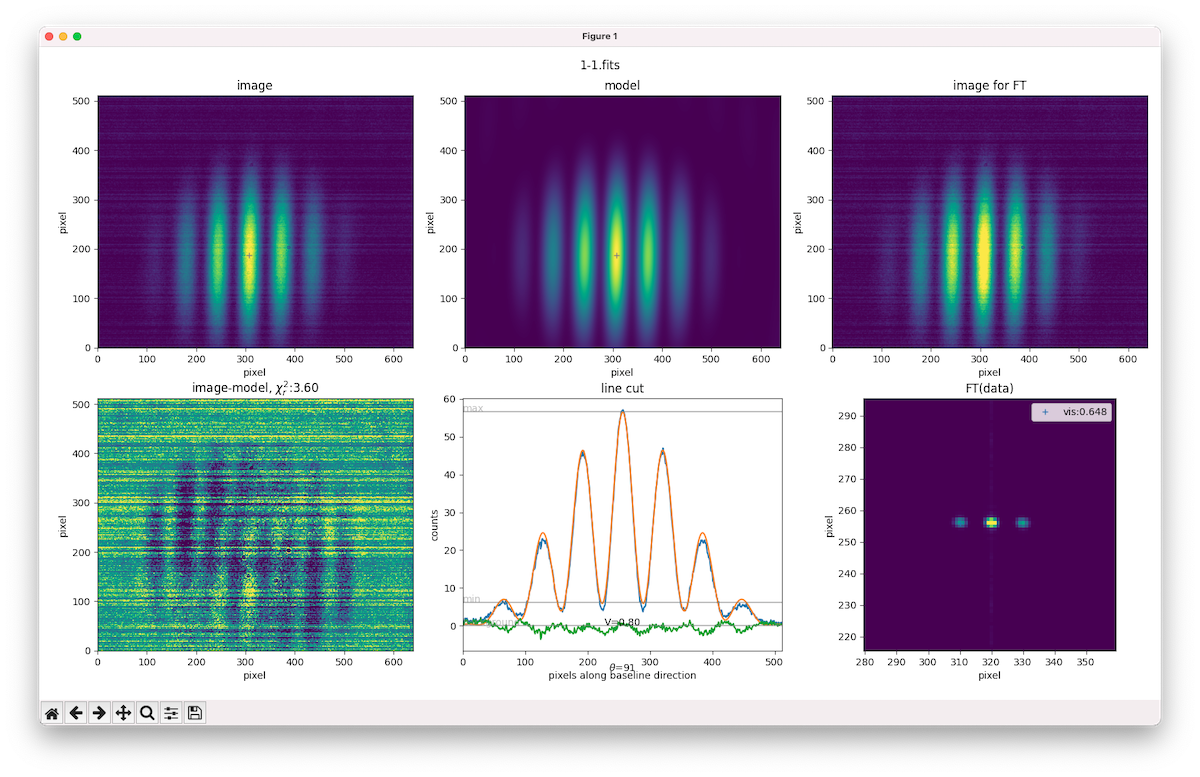
\includegraphics[width=1\textwidth]{widget-fourier.png}
    \caption{Example widget window with the Fourier option turned on.}
    \label{fig:widget-f}
\end{figure}

The result of Fourier transforming an image is shown in Figure \ref{fig:widget-f}. This version of the window can be obtained with the same call to \texttt{widget.py} or \texttt{widget.fit\_fringes()}, but with an extra argument. In the shell case, adding any third argument (e.g. \texttt{f}) will invoke the Fourier panels. In the python terminal, adding \texttt{fourier=True} to \texttt{fit\_fringes()} is needed.

The modified image used in the Fourier transform is shown in the top right panel. If the background is low then this image is identical to the top left one. The lower right panel shows a zoom in of the Fourier transform (the absolute value, here we will not use the phases associated with each frequency). It is an image, because the data are 2d, and the axes are such that the lowest frequencies are represented by pixels at the image center, and more distant pixels are increasingly high frequencies. The highest peak, at the center of the image corresponds to the overall PSF, and the two secondary peaks are the fringes. The orientation of the secondary peaks depends on the angle the fringes are at in the image. The fringes are represented by two peaks because both correspond to the same frequency and orientation.

The peaks for the PSF and fringes in the Fourier transform tell us how much power is in each component, and importantly, the peak for the fringe component is the visibility. The only thing to account for is how strong this peak is relative to the PSF peak, so we first scale the Fourier transform so that the peak in the center for the PSF is equal to 1. Then the visibility is $n_{\rm holes}$ times the peak value (if we added a third hole, the PSF would be brighter, but the original fringe component visibility would not change). Deriving this result is not straightforward \citep[e.g.][section 2.4.3]{2011psi..book.....G}. If we had multiple sets of fringes, we could use a Fourier transform to decompose an image into its Fourier components (i.e. one for each baseline) and measure multiple visibilities at once.

You can explore how the Fourier transform behaves for individual components in the images with one of the notebooks in the \texttt{px-interferometry} package.

Practically, visibility measurements with the Fourier method are more susceptible to low quality data, e.g. if the signal to noise ratio is low background image artefacts can influence the results (e.g. striping at high detector gain). Longer exposures with lower gain should yield better results.

\clearpage
\section{The experiment}

There are many possible measurements that could be made with this experimental setup. The two key ones you should do are:
\begin{itemize}
    \item Demonstrate the effect of bandwidth on coherence. First, estimate the bandwidth of the detector with no filter in place. This means estimating where the fringes become incoherent (e.g. after $n \times \lambda/b$ as in Fig. \ref{fig:coherence}), which then means the ratio of bandwdith to mean wavelength is approximately $\lambda/(2n)$, where $\lambda$ is the mean wavelength of the band. You can derive this result from $(n-1/4)\lambda_1/b = (n+1/4)\lambda_2/b$. You will need to choose a baseline token that results in enough fringes to see this effect, but still has a significant visibility (the example in Fig. \ref{fig:widget2} has $b$ too small.) Show that this coherence problem is significantly reduced when the filters are used.
    \item Measure the angular size of a circular source (i.e. aperture). This means taking visibility measurements with multiple baselines and filters to cover enough range in $b/\lambda$ to constrain the source angular size. Because the source is circular the baseline orientation does not matter. You will need to consider how to estimate uncertainties, and almost certainly need to take multiple sets of measurements and experiment with variables such as exposure time to get reliable results.
    % \item Verify the expected visibility variation with baseline for a binary source. A binary source that is too wide will be resolved out on even the shortest baselines, so a closer binary source is better. In this part you will need to ensure that the baseline holes have close to the same orientation as the binary. 
\end{itemize}

Beyond these some possible options are to:
\begin{itemize}
    \item Use the above method to characterise the shape of a non-rotationally symmetric source. This would involve the same method as for the sources above, but in addition rotating the baseline with respect to the source to measure the size as a function of baseline rotation.
    \item Try repeating the source size measurement, but using Fourier transforms to extract the visibilities from the data. There is an option in the widget to compute a Fourier transform of the data and model, and to estimate the power of the peak frequency from the image. Compare your results from the image-fitting and Fourier methods, if one seems much worse, can it be improved? (e.g. by increasing the exposure time to obtain less noisy images, or by padding the images before the Fourier transform).
    \item Use the three-hole baseline token to take some measurements (e.g. to measure an aperture size and/or shape). This would involve using Fourier transforms as simultaneously fitting multiple fringes will be difficult.
\end{itemize}

\subsection{Basic procedure}

The basic procedure for this experiment is to set things up as you desire, verify the setup is working visually using the image on the screen, and to then save that image. These steps are then repeated as necessary to obtain a full set of images, e.g. across several baselines with different filters. The resulting images are then analysed to obtain visibility measurements, and these visibilities are then used in concert with the baseline length and filter wavelength information to obtain a result.

This result would typically be a plot of baseline vs. $b/\lambda$, and/or a fit to the relevant theoretical curve to obtain an estimate of the source aperture size. An example jupyter notebook for fitting a visibility function to data is included in the \texttt{px-interferometry} package. This notebook also shows how one can take a series of measurements in a systematic sequence, and then restore the saved fitting results to get the values for the plot in an automated way.

You will also need to consider how to incorporate uncertainties on your visibilities, one way to estimate these is to take multiple images for a given baseline/filter.

\subsection{Other considerations}

The experimental setup here is simple, so you will get different visibilities from the fringe fitting and Fourier methods, and when fitted to a function neither will generally result in the theoretical result that the visibility is 1 at the shortest baselines. There are various reasons. For example, we are using a finite bandwidth which means a range of fringe frequencies are actually present, so the fringes lose coherence farther from the center, and this will affect the fringe fitting and Fourier methods differently.

This loss of visibility does not affect the results for source size/separation however, so the amplitude can be simply included as a free parameter in the fitting. For a real astronomical observation these losses still occur, so a typical method is to observe a source that is known to be very small (e.g. a distant but bright giant star) and hence should match the theoretical visibility. This data can then be used to calibrate the science observations of a resolved source. Where your results differ from what is expected, you should consider and discuss possible reasons.

\clearpage
\bibliographystyle{aasjournal}
\bibliography{refs}

\end{document}  